\documentclass[10pt]{beamer}

\usetheme{metropolis}
\setbeamertemplate{itemize subitem}{--}
\setbeamerfont{caption}{size=\footnotesize}
\usepackage{appendixnumberbeamer}

\usepackage{listings}
\lstset{language=C,basicstyle=\footnotesize\ttfamily, backgroundcolor
  = \color{gray!20}} \usepackage{caption}
\captionsetup[lstlisting]{font={small,tt}, labelformat=empty, labelsep=none}

\usepackage{booktabs}
\usepackage[scale=2]{ccicons}

\usepackage{pgfplots}
\usepgfplotslibrary{dateplot}

% Figure's path
\graphicspath{{./figs/}}

\title{Optimization and Profiling of HPC Applications}
\subtitle{using free software resources}
\date{\today}
\author{Emilio J. Padrón González}
 \institute{\href{mailto:emilioj@udc.gal}{\nolinkurl{emilioj@udc.gal}}
   -- \url{http://gac.udc.es/~emilioj}\\Computer Architecture Group
   -- Universidade da Coruña}

\begin{document}

\maketitle

\begin{frame}{Outline}
  \setbeamertemplate{section in toc}[sections numbered]
  \tableofcontents[hideallsubsections]
\end{frame}

\begin{frame}{Contents: Lesson 1 and 2}
  \setbeamertemplate{section in toc}[sections numbered]
  \setbeamertemplate{subsection in toc}[ball unnumbered]
  \tableofcontents[sections={1-2}]
\end{frame}

\begin{frame}{Contents: Lesson 3}
  \setbeamertemplate{section in toc}[sections numbered]
  \setbeamertemplate{subsection in toc}[ball unnumbered]
  \tableofcontents[sections={3}]
\end{frame}


\section{Introduction}

\frame{
  \frametitle{Forms of parallel computing}

  \begin{itemize}
  \item Bit-level parallelism
  \item Instruction-level parallelism (ILP)
  \item Data-level parallelism (DLP)
  \item Task-level parallelism (TLP)
  \end{itemize}
}

\frame{
  \frametitle{A taxonomy of computer architectures}

  Flynn's taxonomy (1966!)

  \begin{description}
  \item[SISD] Single Instruction stream; Single Data stream
  \item[MISD] Multiple Instruction stream; Single Data stream
  \item[SIMD] Single Instruction stream; Multiple Data stream
  \item[MIMD] Multiple Instruction stream; Multiple Data stream
  \end{description}

  \begin{figure}
    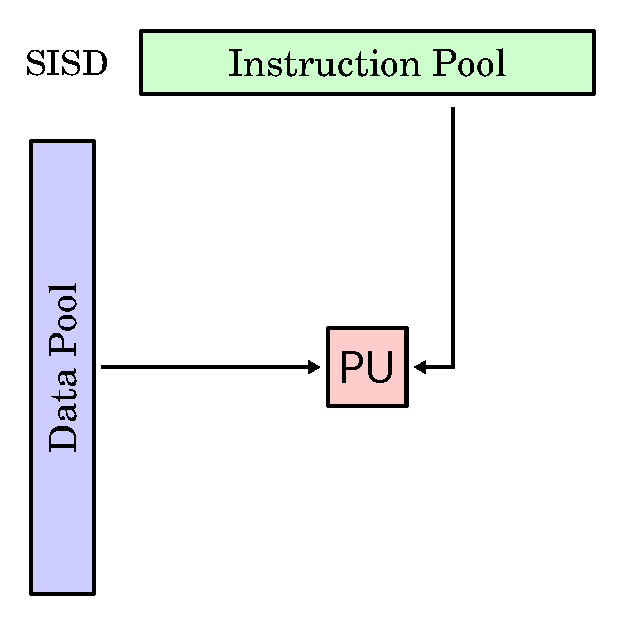
\includegraphics[width=0.25\textwidth]{SISD}~
    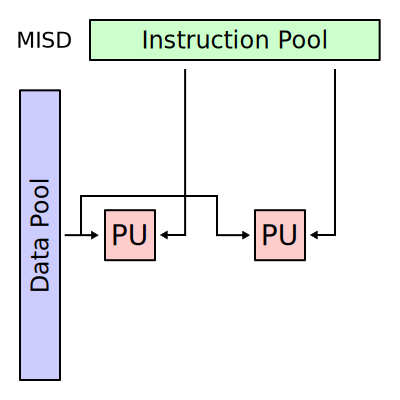
\includegraphics[width=0.25\textwidth]{MISD}~
    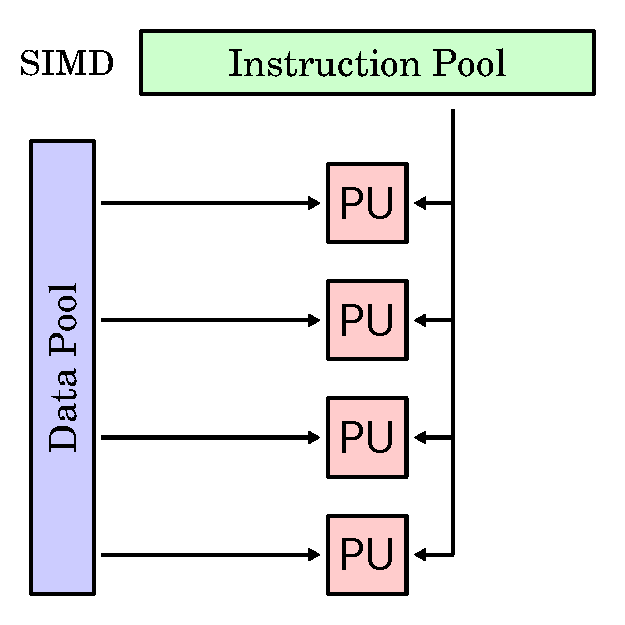
\includegraphics[width=0.25\textwidth]{SIMD}~
    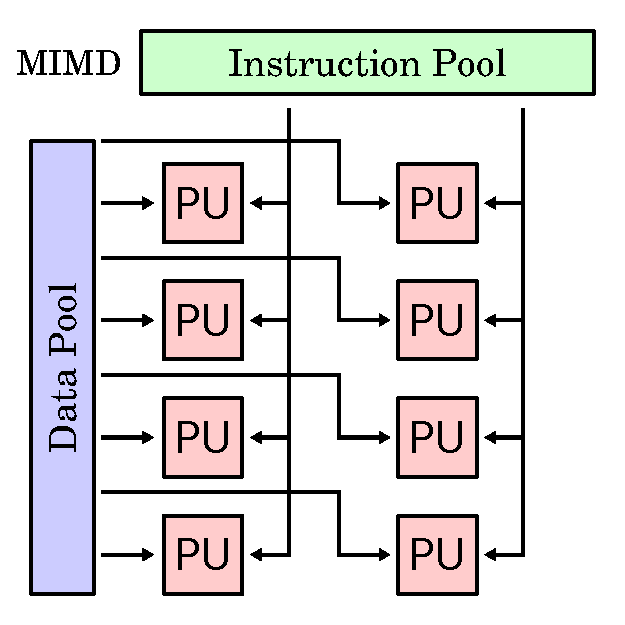
\includegraphics[width=0.25\textwidth]{MIMD}
    \caption{By I, Cburnett, CC BY-SA 3.0,
      \url{https://commons.wikimedia.org/w/index.php?curid=2233537}}
  \end{figure}
}

\frame{
  \frametitle{Parallel processing in Flynn's taxonomy}

  \begin{block}{SISD: exploit ILP}
    \begin{itemize}
    \item Superscalar processors
    \item Pipelining
    \end{itemize}
  \end{block}

  \begin{block}{SIMD: exploit data parallelism}
    \begin{itemize}
    \item Array and Vector processors
    \item Vector extensions in general purpose CPU
    \item GPGPU or similar approaches based on co-processors
    \end{itemize}
  \end{block}

  \begin{block}{MIMD: exploit task parallelism}
    \begin{itemize}
    \item Multicore, multiprocessor and multicomputer architectures
    \end{itemize}
  \end{block}

}

\frame{
  \frametitle{Typical performance metrics}

  \begin{itemize}
  \item CPU
    \begin{itemize}
    \item MIPS
    \item FLOPS (usually GFLOPs/sec)
    \end{itemize}
  \item Memory \& I/O
    \begin{itemize}
    \item Latency (time units)
    \item Bandwith/Throutput (usually GBs/sec)
    \end{itemize}
  \end{itemize}
}

\frame{
  \frametitle{Performance characterization}

  Identifying the dominant bottleneck:
  \begin{itemize}
  \item Compute bound (aka CPU bound)
  \item Memory bound
    \begin{itemize}
    \item Cache bound
    \end{itemize}
  \item I/O bound
  \end{itemize}

  Obviously, in terms of velocity:
  \begin{itemize}
  \item[] CPU > Cache (L1 > L2 > L3) > Mem > I/O
  \end{itemize}

}

% Good explanation from https://stackoverflow.com/questions/868568/what-do-the-terms-cpu-bound-and-i-o-bound-mean
% CPU Bound means the rate at which process progresses is limited by the speed of the CPU. A task that performs calculations on a small set of numbers, for example multiplying small matrices, is likely to be CPU bound.

% I/O Bound means the rate at which a process progresses is limited by the speed of the I/O subsystem. A task that processes data from disk, for example, counting the number of lines in a file is likely to be I/O bound.

% Memory bound means the rate at which a process progresses is limited by the amount memory available and the speed of that memory access. A task that processes large amounts of in memory data, for example multiplying large matrices, is likely to be Memory Bound.

% Cache bound means the rate at which a process progress is limited by the amount and speed of the cache available. A task that simply processes more data than fits in the cache will be cache bound.

% I/O Bound would be slower than Memory Bound would be slower than Cache Bound would be slower than CPU Bound.

% The solution to being I/O bound isn't necessarily to get more Memory. In some situations, the access algorithm could be designed around the I/O, Memory or Cache limitations.

\frame{
  \frametitle{The Roofline Model}

  \metroset{block=fill}

  \begin{block}{Basic Roofline Model}
    Bounds Floating-point performance as a function of
    \begin{itemize}
    \item machine peak performance (GFLOPs/sec)
    \item machine peak bandwidth (GBytes/sec)
    \item arithmetic intensity (FLOPs/Byte) \hfil \alert{\small <--- core concept}
    \end{itemize}
  \end{block}

  \begin{figure}
    \begin{overprint}
      \onslide<1>\centering
      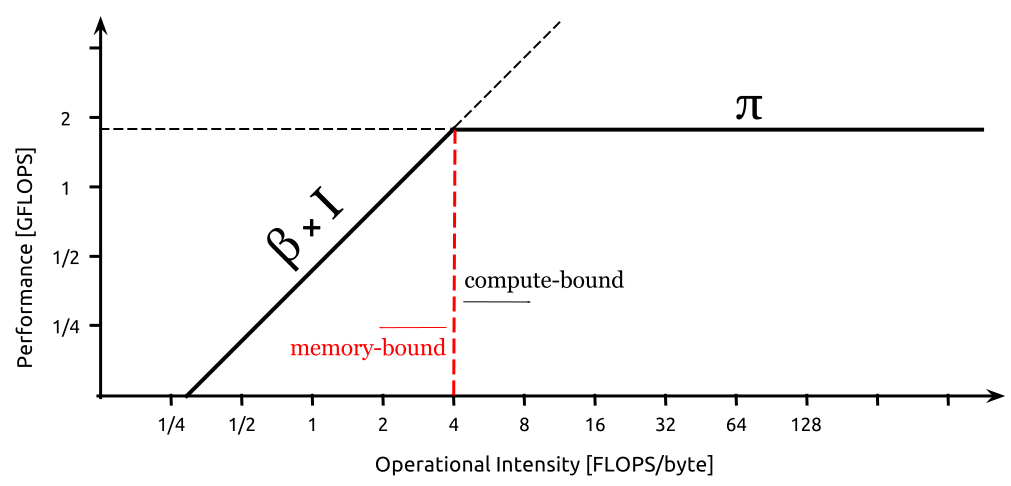
\includegraphics[width=.7\textwidth]{naive_roofline_model}
      \onslide<2>\centering
      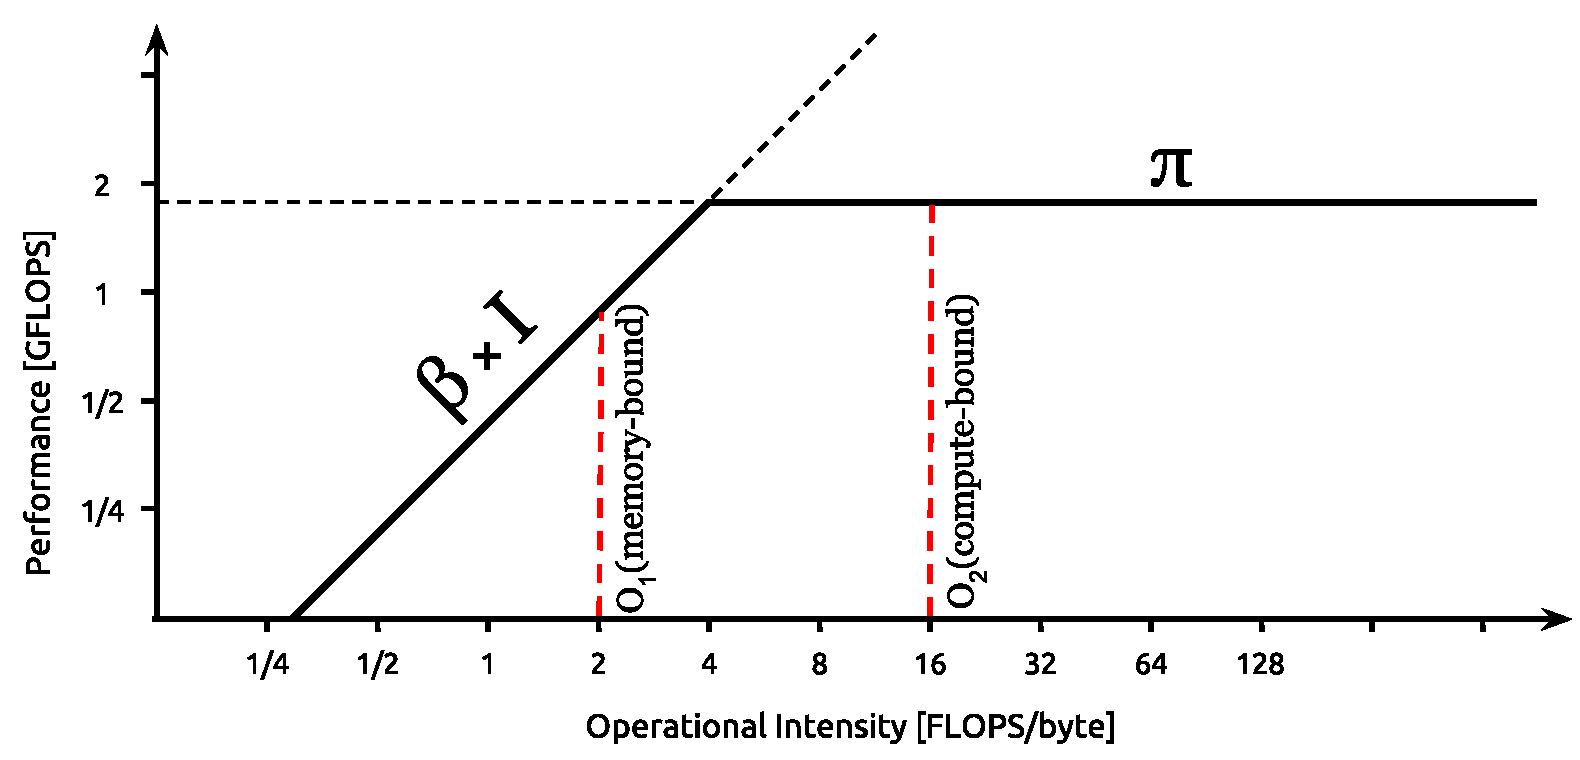
\includegraphics[width=.7\textwidth]{naive_roofline_model2}
    \end{overprint}
    \caption{Original image by Giu.natale, CC BY-SA 4.0, modified by me
      \url{https://commons.wikimedia.org/w/index.php?curid=49641351}}
  \end{figure}
}

\frame{
  \frametitle{Expanding the roofline plot}

  \begin{figure}\vspace*{-0.7cm}
    
\includegraphics[width=.5\textwidth]{roofline_model_bandwith_ceilings}~
    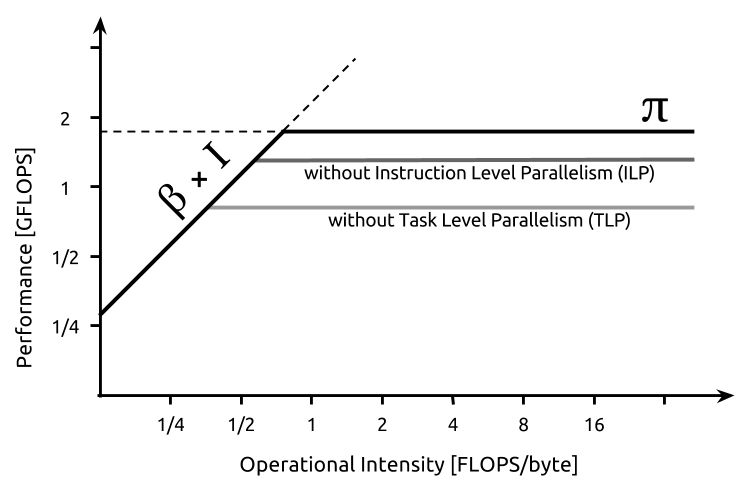
\includegraphics[width=.5\textwidth]{roofline_model_in-core_ceilings}
    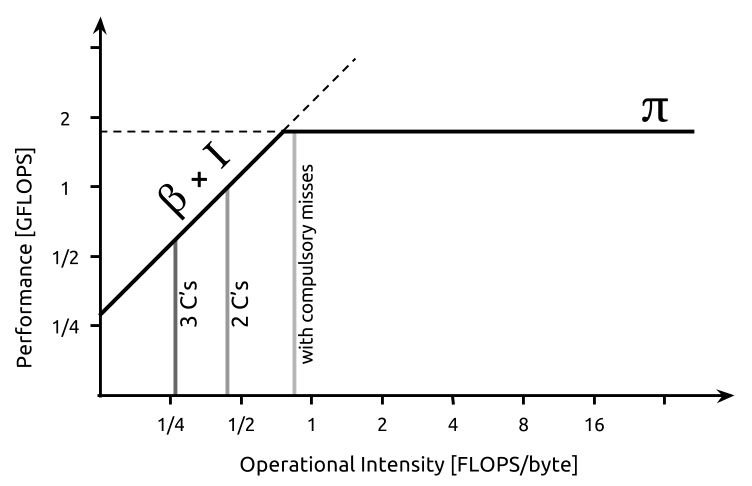
\includegraphics[width=.5\textwidth]{roofline_model_locality_walls}
    \caption{By Giu.natale - Own work, CC BY-SA 4.0,
      \url{https://commons.wikimedia.org/w/index.php?curid=49593615}
      \url{https://commons.wikimedia.org/w/index.php?curid=49593667}
      \url{https://commons.wikimedia.org/w/index.php?curid=49593835}
    }
  \end{figure}
}

\frame{
  \frametitle{Roofline model: an intuitive visual performance model}

  \begin{itemize}
  \item Provides performance estimation
    \begin{itemize}
    \item of a given compute kernel or application
    \item on a specific platform
    \end{itemize}

    \metroset{block=fill}
    \begin{block}{Visual and intuitive: key information at a glance}
      \begin{itemize}
      \item[\checkmark] Shows inherent hardware limitations
      \item[\checkmark] Highlights potential benefit and priority of
        optimizations
      \end{itemize}
    \end{block}
  \end{itemize}

  \begin{figure}
    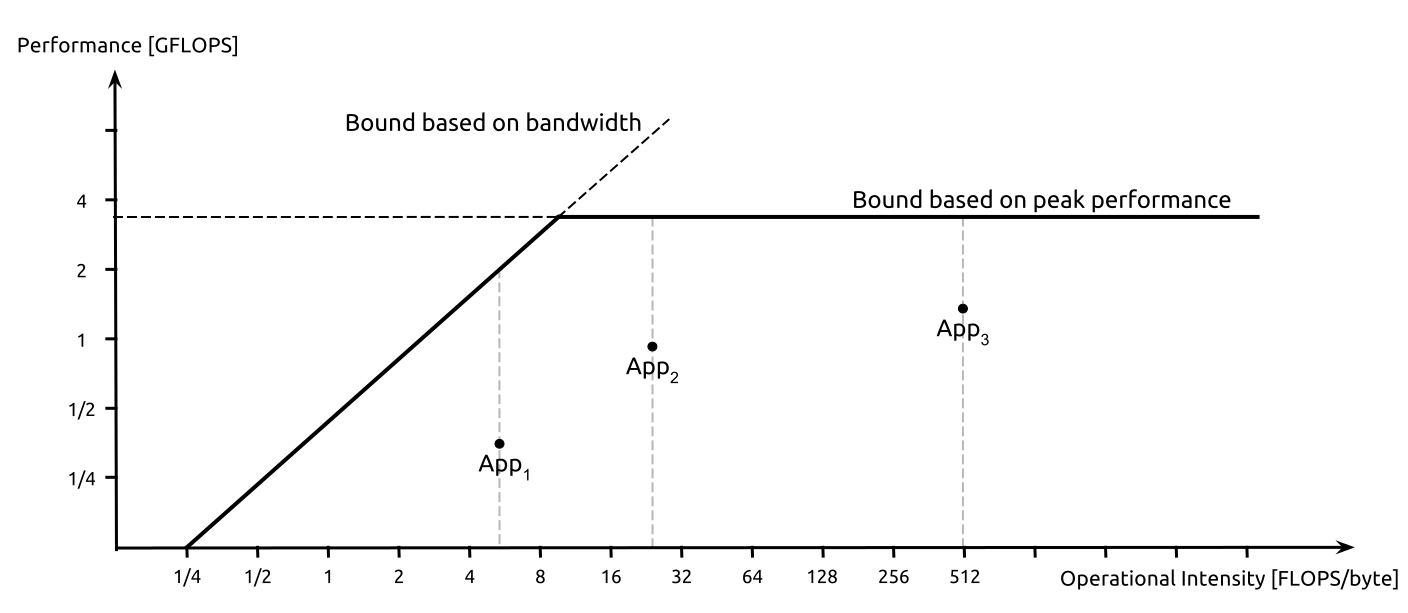
\includegraphics[width=.7\textwidth]{naive_roofline_model_example}
    \caption{By Giu.natale - Own work, CC BY-SA 4.0,
      \url{https://commons.wikimedia.org/w/index.php?curid=49641314}}
  \end{figure}
}

\section{Optimization and Profiling of Sequential Code}

\frame{
  \frametitle{\insertsectionhead}

  Main tools we'll use in this course:
  \begin{description}
  \item[Compiling] ~\\
    GNU Compilers: gcc, g++, gfortran
  \item[Debugging] ~\\
    gdb
  \item[Profiling and performance analysis] ~\\
    gprof, gcov, valgrind, gperftools
  \item[Performance characterization] ~\\
    Berkeley Lab's CS Roofline Toolkit
  \end{description}
}

\subsection{Compiler optimizations}

\frame{
  \frametitle{Looking at the compiler}
  How can the compiler help us to achieve efficient binaries from our
  source codes for a specific platform?
  \begin{itemize}
  \item Optimization options

    {\small \tt gcc [-Q] --help=optimizers}

    \makebox[0pt][r]{\tiny last gcc doc ->\hspace*{0.15cm}}{\scriptsize
      \url{http://gcc.gnu.org/onlinedocs/gcc/Optimize-Options.html}}

    \makebox[0pt][r]{\tiny gcc 7.2 doc ->\hspace*{0.15cm}}{\scriptsize
      \url{http://gcc.gnu.org/onlinedocs/gcc-7.2.0/gcc/Optimize-Options.html}}\\[0.5cm]

  \item Target-specific / machine-dependent options (x86)

    {\tt gcc [-Q] --help=target}

    \makebox[0pt][r]{\tiny last gcc doc ->\hspace*{0.15cm}}{\scriptsize
      \url{http://gcc.gnu.org/onlinedocs/gcc/x86-Options.html}}

    \makebox[0pt][r]{\tiny gcc 7.2 doc ->\hspace*{0.15cm}}{\scriptsize
      \url{http://gcc.gnu.org/onlinedocs/gcc-7.2.0/gcc/x86-Options.html}}
  \end{itemize}
  }

\frame{
  \frametitle{Compiler machine-dependent options (x86)}

  (a.k.a. {\it `-m'} options)

  \begin{description}
  \item[{\tt -march={\it cpu-type}}] Generate instructions for that
    machine type\\
    E.g. {\tt native|x86-64|haswell|\ldots}
  \item[{\tt -mtune={\it cpu-type}}] Tune generated code for that
    machine type
  \item[{\tt -mavx -mavx2\ldots}] Enable the use of extended
    instruction sets (vector instructions, mostly)
  \end{description}

  \vfill
  -> {\footnotesize Check target specific options with:
    {\tt gcc -Q -march=native --help=target}}
}

\frame{
  \frametitle{Compiler optimization levels}

  In a nutshell: \hfil (each level includes the previous)
  \begin{description}
  \item[{\tt -O0}] [Default] No optimization. Reduces compilation time
    and make debugging produce the expected results.
  \item[{\tt -O/-O1}] Optimize. Tries to reduce code size and execution
    time, avoiding optimizations that take high compilation time.
  \item[{\tt -O2}] Optimizes even more.
  \item[{\tt -O3}] Optimizes yet more.
  \item[{\tt -Ofast}] Enables {\tt -ffast-math}, optimizations that
    are not valid for all standard-compliant programs.

    Additionally, Fortran-specific {\tt -fstack-arrays}, unless {\tt
      -fmax-stack-var-size} is specified, and {\tt
      -fno-protect-parens}.
  \end{description}

  --> {\footnotesize Check specific options being enable/disable at
    each level for your compiler version with {\tt gcc -Q -O2
      --help=optimizers} (or in the doc)}
}

\frame{
  \frametitle{Some key optimizations at compilation time}

  \begin{itemize}
  \item Inlining
  \item Loop optimizations
    \begin{itemize}
    \item Vectorization
    \item Loop peeling
    \item Loop unrolling
    \end{itemize}
  \item Interprocedural optimizations
  \item Profile-guided optimizations
  \end{itemize}
}

\begin{frame}[fragile]{Vectorization}

  \begin{description}
  \item[Vectorization] Form of SIMD which allows us to crunch multiple
    values in one CPU instruction
  \end{description}

  => Especially useful to \underline{optimize loop execution} (but not
  exclusively)

  \begin{columns}
    \column{0.45\textwidth}{
      \begin{lstlisting}[gobble=8,caption={Sequential loop}]
        float A[32], B[32], C[32];

        for (i=0; i<32; i++)
          C[i] = A[i] + B[i];
          // 32 float ADD operations
      \end{lstlisting}
    } \
    \column{0.55\textwidth}{
      \begin{lstlisting}[gobble=8,caption={Vectorized pseudocode}]
        float A[32], B[32], C[32];

        for (i=0; i<32; i+=8)
          C[i:i+7] = A[i:i+7] + B[i:i+7];
          // vectorization factor: 8
          // => 4 vector float ADD ops
      \end{lstlisting}
    }
  \end{columns}
\end{frame}

\frame{
  \frametitle{Vectorization: Intel SIMD extensions}

  \begin{figure}
    \includegraphics{avx_regs}
    \caption{x86-64 Vector Registers}
  \end{figure}
  \begin{itemize}
  \item AVX-512 (ZMM0--ZMM31)
  \item AVX/AVX2 (YMM0--YMM31) \quad \alert{\small --> AVX2 in FT2's Haswell procs}
  \item SSE (XMM0--XMM31)
  \end{itemize}
}

\begin{frame}[fragile]{Vectorization: x86-64 vector operations}

  \begin{itemize}
  \item Intrinsic C-like functions to access vector instructions\\
    e.g.\\[0.2cm]
    \begin{columns}
      \column{0.3\textwidth}{
        {\bf AVX asm instruction}\\
        \begin{lstlisting}[gobble=9]
          vmovaps ymm, m256
        \end{lstlisting}
      } \
      \column{0.73\textwidth}{
        {\bf Intrinsic function}\\
        \begin{lstlisting}[gobble=9]
          __m256 _mm256_load_ps (float const *mem_addr)
          #include <immintrin.h>
        \end{lstlisting}
      }
    \end{columns}

  \item[] \hspace*{-0.7cm} \mbox{\scriptsize \alert{(doc)} Intrinsics Guide: \url{http://software.intel.com/sites/landingpage/IntrinsicsGuide}}\\
  \item SIMD instructions typically require:
    \begin{itemize}
    \item aligned data
    \item no pointer aliasing
    \end{itemize}
  \end{itemize}

  \pause

  \begin{columns}
    \column{0.35\textwidth}{
      \begin{alertblock}{Writing vectorized code}
        \begin{itemize}
        \item hard
        \item error-prone
        \end{itemize}
      \end{alertblock}
    }
    \column{0.01\textwidth}{
      \mbox{-->}
    }
    \column{0.5\textwidth}{
      \begin{exampleblock}{Autovectorization}
        \structure{\checkmark} Let compiler do it for you
      \end{exampleblock}
    }
  \end{columns}
\end{frame}


\frame{
  \frametitle{GCC autovectorization compiler flags}

  \begin{description}
  \item[{\tt -ftree-loop-vectorize}] Enable loop vectorization
  \item[{\tt -ftree-slp-vectorize}] Enable basic block vectorization (SLP)
  \end{description}
  \begin{itemize}
  \item Both flags are enabled by default in {\tt -O3} and {\tt
      -Ofast}, and are also enabled with {\tt -ftree-vectorize}
  \item {\tt Ofast}'s additional (unsafe) math optims may help autovect
  \item Do not forget {\tt -march=native}
  \item Reports: list (not) vectorized loops + extra info
    {\tt -fopt-info-vec}\\
    {\tt -fopt-info-vec-missed}\\
    {\tt -fopt-info-vec-all} {\footnotesize(detailed autovect process)}
  % \item Additionally:
  %   \begin{description}
  %   \item[{\tt -fvect-cost-model=[unlimited|dynamic|cheap]}] Specifies
  %     the cost model for vectorization
  %     %(default O3/Ofast: {\tt dynamic})
  %   \item[{\tt -fsimd-cost-model=[unlimited|dynamic|cheap]}] Specifies
  %     the vectorization cost model for code marked with a simd
  %     directive
  %     %(default O3/Ofast: {\tt unlimited})
  % \end{description}
  \end{itemize}
}

\frame{
  \frametitle{GCC autovectorization compiler directives}

  GCC Vectorization
  pragmas~\footnote{\url{http://gcc.gnu.org/onlinedocs/gcc/Loop-Specific-Pragmas.html}}:
  \begin{itemize}
  \item {\tt \#pragma GCC ivdep}
    \begin{itemize}
    \item programmer asserts no loop-carried dependencies
    \end{itemize}
  \end{itemize}
}

\frame{
  \frametitle{Profile-guided optimizations}
}

\frame{
  \frametitle{Some good coding practices to help compilers}

  \begin{itemize}
  \item restricted
  \end{itemize}
}

\subsection{Evaluating execution time and detecting hot spots}

\frame{
  \frametitle{Profiling}

  \begin{itemize}
  \item Profiling tools help you analyze your code's performance:
    \begin{itemize}
    \item how often each line of code executes
    \item what lines of code are actually executed
    \item how much computing time each section of code uses
    \end{itemize}
  \end{itemize}
}

\frame{
  \frametitle{GPROF: the GNU Profiler}

}

\subsection{Evaluating memory usage}

\frame{
}

\subsection{Evaluating cache usage and performance}

\frame{
}


\subsection{The \emph{roofline} model}

\frame{
}

\subsection{Strategies to detect vectorization and parallelization
  opportunities}

\frame{
}


\section{Optimization and Profiling of Parallel Code}

\frame{
  \frametitle{\insertsectionhead}

  \begin{itemize}
  \item Paraver, Extrae y Dimemás
  \item ompP
  \end{itemize}
}

\subsection{Shared memory (OpenMP)}

\frame{
}

\subsubsection{Load balancing optimization}

\frame{
}

\subsubsection{Communication analysis and optimization}

\frame{
}

\subsection{Distributed memory (MPI)}

\frame{
}

\subsubsection{Load balancing optimization}

\frame{
}

\subsubsection{Communication analysis and optimization}

\frame{
}

\subsection{Hybrid parallel programming: shared + distributed Mem}

\frame{
}

\subsubsection{Load balancing optimization}

\frame{
}

\subsubsection{Communication analysis and optimization}

\frame{
}

\end{document}
